\documentclass{article}
\usepackage[a4paper,top=2cm,bottom=2cm,left=2cm,right=2cm]{geometry}
\usepackage[english]{babel}
\usepackage[utf8]{inputenc}
\usepackage{fancyhdr}
\usepackage{float}
\usepackage{graphicx}
\usepackage{wrapfig}
\usepackage{siunitx} %per scrivere il simbolo °
\usepackage{verbatim} %per i commenti1
\usepackage{subfig}
\usepackage{amsmath}
\usepackage{algorithm}
\usepackage{algpseudocode}
\setcounter{secnumdepth}{3}
\setcounter{tocdepth}{6}
\usepackage{multirow}
\newcommand{\minitab}[2][l]{\begin{tabular}#1 #2\end{tabular}}
\usepackage{rotating}
\usepackage{xfrac}
\usepackage{cite}

\DeclareMathOperator*{\argmax}{arg\,max}
\DeclareMathOperator*{\argmin}{arg\,min}

%\usepackage{booktabs,array}
%\usepackage{tikz}

%\usepackage{tabularx}

%\usepackage{chngcntr}
%\counterwithin{table}{section}

%------------------------------ colors
\usepackage[usenames,dvipsnames,table]{xcolor} % use colors on table and more
\definecolor{333}{RGB}{51, 51, 51} % define custom color
\definecolor{background}{RGB}{248, 248, 255}
\definecolor{comment}{RGB}{17,167,5}
\definecolor{keyword}{RGB}{195,47,8}
\definecolor{string}{RGB}{142,195,0}
\definecolor{number}{RGB}{90,84,84}
\definecolor{identifier}{RGB}{0,90,201}

%------------------------------ source code
\usepackage{listings}

\lstset{
  basicstyle=\footnotesize\sffamily,
  commentstyle=\itshape\color{gray},
  captionpos=b,
  frame=shadowbox,
  language=HTML,
  rulesepcolor=\color{333},
  tabsize=2
}

\lstdefinestyle{code}{
  backgroundcolor=\color{background},
  basicstyle=\footnotesize\sffamily,
  commentstyle=\color{comment},
  frame=L,
  identifierstyle=\color{identifier},
  keywordstyle=\color{keyword},
  numbers=left,
  numbersep=10pt,
  numberstyle=\tiny\color{number},
  stringstyle=\color{string},
  showstringspaces=false,  
  stepnumber=1,
  tabsize=2
}

\title{\textbf{Report about Lab4}} % Title
\author{Raffaele \textsc{Di Nardo Di Maio} 1204879} % Author name
\date{\today}

\begin{document}
\begin{minipage}{.20\textwidth}
  
\includegraphics[height=3cm]{../Icon4}
\end{minipage}\begin{minipage}{.20\textwidth}
  \begin{table}[H]
  \begin{tabular}{l}
  \scshape{\Large{Computer Engineering Master Degree}} \\
  \hline \\
  \scshape{\Large{Computer Vision}} \\
  \end{tabular}
  \end{table}
\end{minipage}
{\let\newpage\relax\maketitle}

\section{Goal of the experience}
The goal of this lab experience was to detect a road lane and a street signal in an image, highlighting them respectively with red and green colors. Their extraction was done by using the Canny edge detector and Hough transforms and by tuning their parameters.
\section{Code Organization}
The code of this lab is organized in ten main files (for which I provide also the documentation through doxygen):
\begin{itemize}
\item{\textbf{Lab4.cpp} and its header file \textbf{Lab4.h}.\\
They are associated to \textit{main()} where an instance of \textit{StreetDetector()} is created and its function \textbf{detect()} is called.}
\item{\textbf{StreetDetector.cpp} and its header file \textbf{StreetDetector.h}.\\
These are used to create the class \textit{StreetDetector}. Its main function is called \textbf{detect()} and it creates all the windows for the Canny detector and Hough transforms, creating objects of the classes that implement them. In this function, the main flow of the program is managed. This is organized in two main phases:
\begin{enumerate}
\item{\textbf{Detection of the street}.\\
On screen there are two windows at the same time (Canny edge detection and Hough lines transform). By updating the first one, the second one is also affected by these changes. When one key, between 'q', 'ESC' and '\textbackslash{r}', is pressed by user, the last image in the Hough lines window is used for the next phase.
}
\item{\textbf{Detection of the signal}.\\
Using the previously computed image, a new window is created for Hough circles transform.
}
\end{enumerate}
}
\item{\textbf{CannyDetector.cpp} and its header file \textbf{CannyDetector.h}.\\
These are used to create the class \textit{CannyDetector}, that performs the Canny edge detection.}
\item{\textbf{HoughLinesDetector.cpp} and its header file \textbf{HoughLinesDetector.h}.\\
These are used to create the class \textit{HoughLinesDetector}, that performs Hough transform detection for lines and highlights in red a triangle in the image. This is obtained by the two most significant detected lines.}
\item{\textbf{HoughCirclesDetector.cpp} and its header file \textbf{HoughCirclesDetector.h}.\\
These are used to create the class \textit{HoughCirclesDetector}, that performs Hough transform detection for circles and highlights in green the most significant circle in the image, among all detected circles.}
\end{itemize}
\section{Command line parameters}
The program needs to have, as command line argument, the path of the image ( including its name) on which you want to detect the street and the signal. 
\section{Experimental results}
In the following part there are the resulting images used in my workflow:
\begin{enumerate}
\item{\textbf{Parameters evaluation for Canny detection and Hough lines transform}.\\
Before applying the Canny Detection, to reduce hysteresis thresholds values, I apply a Blur filter of size 9x9. After this smoothing step, I apply the Canny Detector and, after that, the Hough lines transform. The most significant parameters of these detectors are respectively the first threshold and the angle resolution. 
Through Hough Transform, I found the two most significant lines (e.g. Figure \ref{result_lines}). Then evaluating their equations, I compute the three corners, that defines the triangle of the street, and I draw it through \textit{cv::fillPoly()} function.
}
\item{\textbf{Parameters evaluation for Hough circles transform}.\\
The most significant parameters of Hough circles transform are max radius, if we consider a fixed minimum radius of 1, and the second method parameter. By changing second method parameter, in fact, the range of maximum radii, that correctly highlights the signal, changes.  
}
\end{enumerate}
In Table \ref{param}, there are the parameters I used to obtain a good detection of the road lane and the signal. In Figure \ref{result} there is the image, obtained by my program, with detected street and signal. The specified parameters are set at object construction.
\begin{table}[h]
\centering
\begin{tabular}{|c|l|c|}
\hline
\multirow{2}{*}{Canny Detector}&{$threshold_1$}&{$[0.0, 157.0]$}\\
\cline{2-3}
&{$threshold_2$}&{$200$}\\
\hline
\multirow{3}{*}{Hough Lines Detector}&{\textit{distance resolution}}&{$1$}\\
\cline{2-3}
&{\textit{angle resolution}}&{$\frac{37\cdot \pi}{150}$}\\
\cline{2-3}
&{accumulator threshold}&{[0,14]}\\
\hline
\multirow{3}{*}{Hough Circles Detector}&{\textit{minimum distance}}&{$69.0$}\\
\cline{2-3}
&{\textit{parameter 1}}&{$30.0$}\\
\cline{2-3}
&{\textit{parameter 2}}&{$23.0$}\\
\cline{2-3}
&{\textit{minimum radius}}&{$1$}\\
\cline{2-3}
&{\textit{maximum radius}}&{$[10,21]$}\\
\hline
\end{tabular}
\caption{Estimated detected parameters that highlight the signal and the street.}\label{param}
\end{table}
\begin{figure}[h]
\begin{center}
  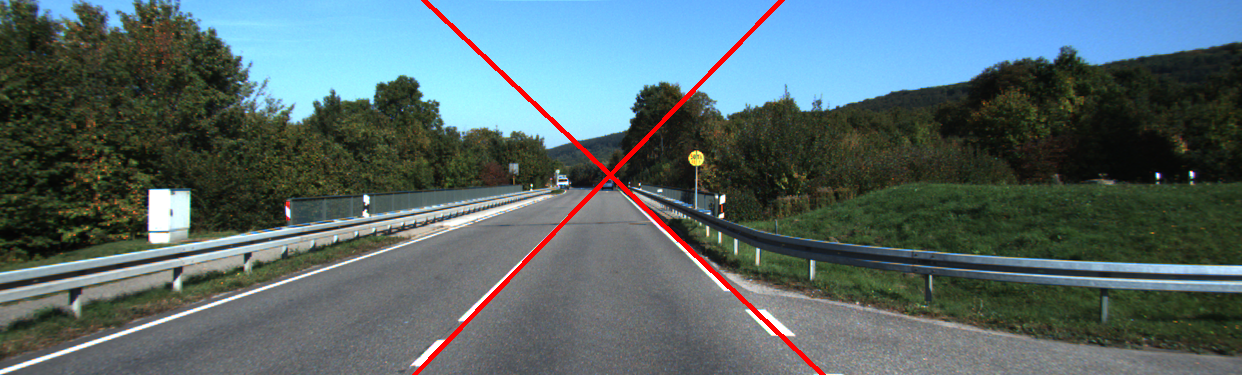
\includegraphics[scale=0.38]{result_lines}\\ 
  \caption{\footnotesize{Image with highlighted most significant lines.}}\label{result_lines} 
\end{center} 
\end{figure}
\begin{figure}[h]
\begin{center}
  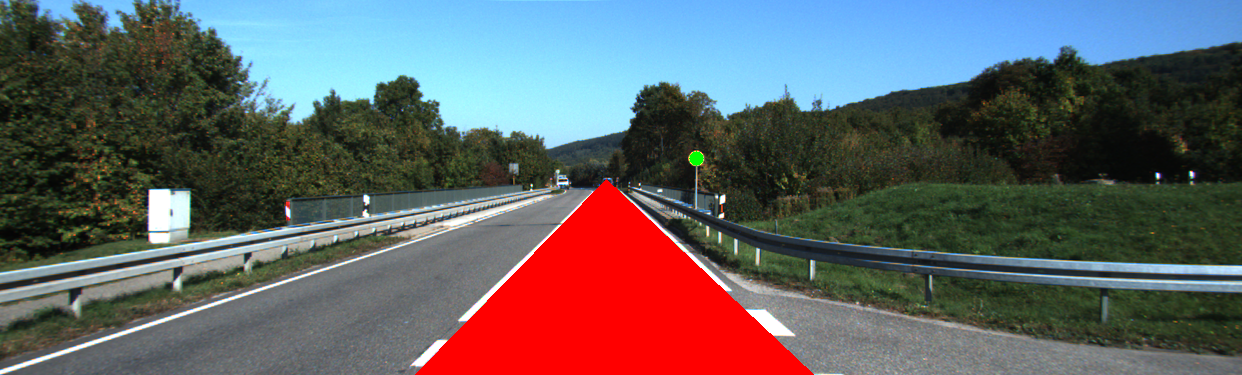
\includegraphics[scale=0.38]{result}\\ 
  \caption{\footnotesize{Image with highlighted street in red and signal in green.}}\label{result} 
\end{center} 
\end{figure}

\end{document}
